% !TeX encoding=utf8
% !TeX spellcheck = de_CH_frami

\chapter{Ausgangslage}

In der heutigen Zeit mit immer komplexer werdenden Geschäftsfeldern und Märkten ist \gls{acr:BPM} ein essentieller Bestandteil kleiner, mittlerer und grosser Unternehmen. \gls{acr:BPM} bietet den Unternehmen viele essentielle Vorteile. Diesen Vorteilen gegenüber stehen jedoch die Aufwände, um \gls{acr:BPM} konsequent umzusetzen und anschliessend weiter zu pflegen.

Vor allem im Industrie-Zweig ist das \gls{acr:IOT} seit längerer Zeit ein wichtiger Bestandteil des Unternehmens. Mit der zunehmenden Verbreitung und Akzeptanz wird der Nutzen des \gls{acr:IOT} zunehmend auch in anderen Wirtschaftszweigen und im Privat- / Heimandwenderbereich entdeckt und genutzt.

Durch die zunehmende Ausbreitung ergeben sich nun zwei Fragestellungen.

\begin{itemize}
\itemBfText{Wie sieht die Kommunikation mit / innerhalb des \gls{acr:IOT} in Zukunft aus?}{Bisher wird das Internet der Dinge eher im Rahmen der Kommunikation von zwei oder mehreren Dingen, beziehungsweise Maschinen betrachtet. Bei gewissen Anwendungsfällen ist jedoch die Integration des Menschen in den Kommunikationsprozess von Vorteil, beziehungsweise sogar unerlässlich. Durch die Einbindung des Menschen ergeben sich dann im Gegenzug viele neue mögliche Einsatzzwecke und Anwendungsgebiete. Als Stichworte sind hier Reporting, Datenanalyse, Datenauswertung, Datenvisualisierung und Entscheidungsfindung zu nennen.}
\itemBfText{Wie wird das \gls{acr:IOT} in die bestehenden Geschäftsprozesse integriert?}{\gls{acr:IOT} Anwendungen / Lösungen wurden bisher oft in einem isolierten Kontext betrachtet. Spätestens nach Inbetriebnahme der Lösung stellt sich früher oder später die Frage, wie das ganze nun in (evtl. bestehende) Geschäftsprozesse integriert werden kann.}
\end{itemize}
\newpage
Eine Möglichkeit um die Problemstellung der ersten Frage zu lösen, wäre über die Beantwortung / Lösung der zweite Frage. Dies würde bedeuten, dass die Kommunikation zwischen Geräten und Menschen über die Implementation / Anbindung von Geschäftsprozessen bewerkstelligt werden könnte.

Diese beiden Fragestellungen stellen sich nicht nur für den Geschäftsbereich, sondern auch im Privatbereich. \gls{acr:IOT}-Endgeräte, beziehungsweise "`Dinge"' halten immer mehr auch im Privatbereich Einzug. Dabei handelt es sich oftmals um Produkte aus dem Bereich der Heimautomatisierung. Bei der Heimautomatisierung geht es ebenfalls um die Automatisierung / Steuerung von Abläufen. Im weitesten Sinn handelt es sich somit auch um Geschäftsprozesse.

Diese Arbeit soll aufzeigen, was es für Heimanwender für Möglichkeiten gibt um solche "`Geschäftsprozesse"' im Bereich der Heimautomatisierung zu realisieren.







\section{Business Process Managemnt (BPM)} \label{sec:Ausg:BPM}
Dieses Kapitel erläutert die wichtigsten Informationen rund um das Management von Geschäftsprozessen (Business Process Management).

Jedes Unternehmen hat Business Prozesse. Prozesse sind Abläufe, beziehungsweise Abfolgen von Schritten und Tätigkeiten. Diese Schritte müssen in einer bestimmten logischen Reihenfolge von einem Individuum oder einer Maschine ausgeführt werden. Jeder Prozess dient einem bestimmten Zweck und dient dazu ein vordefiniertes Ziel zu erreichen \cite{E:SearchCIO:Def:BPM}.

Je nach Art und Grösse des Unternehmens können diese Business Prozesse unterschiedliche Komplexitäten und Stellenwerte aufweisen. Oft werden die Business Prozesse mit der Zeit (und dem Wachstum des Unternehmens) immer grösser, vielfältiger und komplizierter.

Daher ist es in der Regel sinnvoll einen strukturierten Ansatz zur Verwaltung / Pflege / Umsetzung der Business Prozesse zu verwenden. Die nachfolgende Auflistung zeigt einige Gründe für die Verwendung eines strukturierten Ansatzes.

\begin{itemize}
\item Schwierigkeiten die Übersicht über die laufenden / offenen Prozesse zu behalten.
\item Prozessschritte können vergessen oder in falscher Reihenfolge durchgeführt werden.
\item Prozessschritte können unterschiedlich durchgeführt werden.
\item Redundante Arbeitsschritte
\item Wissensübertragung schwierig.
\item Hoher Aufwand für die Einarbeitung
\end{itemize}

\newpage
\gls{acr:BPM} ist eine Methode, beziehungsweise ein strukturierter und systematischer Ansatz um Business Prozesse (und Workflows) effektiver, effizienter und flexibler zu gestalten.
Einige der wichtigsten Ziele von \gls{acr:BPM} werden nachfolgend aufgelistet.

\begin{itemize}
\item Reduktion, beziehungsweise Abstraktion, der Komplexität der Business Prozesse
\item Minimierung von menschlichen Fehlern.
\item Stakeholder können sich auf ihre eigentliche Rolle konzentrieren.
\end{itemize}

Früher hatte \gls{acr:BPM} primär zum Ziel Prozesse zu visualisieren, zu automatisieren und dadurch die Effizienz zu steigern. Heutige \gls{acr:BPMS} bieten inzwischen viele zusätzliche Funktionalitäten an. Dazu gehören zum Beispiel End-User-Portale, Integration mit unterschiedlichsten Systemen, Analyse Möglichkeiten und Mobile-Fähigkeit.


\subsection{Lebenszyklus / Phasen}
Innerhalb von \gls{acr:BPM} gibt es die nachfolgende aufgezeigten Phasen.

\begin{figure}[H]
  \centering
  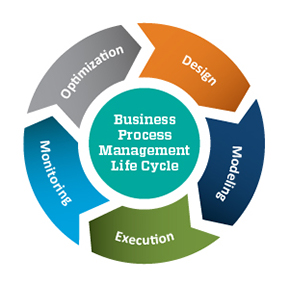
\includegraphics[width=8cm]{./images/BPMN_Lifecycle}
  \captionsource{Lebenszyklus / Phasen von BPMN}{\url{http://legatoconsulting.ca/solutions.html}}
\end{figure}

\begin{itemize}
\itemBfText{Design}{In der Design-Phase werden bestehende und mögliche neue Prozesse identifiziert. Dabei wird der Prozess im Ist-Zustand modelliert.}
\itemBfText{Modelling}{In der Modellierungs-Phase wird der Ist-Prozess analysiert und auf verschiedene Verbesserungsmöglichkeiten hin überprüft.}
\itemBfText{Execution}{In der Execution-Phase wird der verbesserte / veränderte Prozess im Tagesgeschäft umgesetzt. Dies kann, muss aber nicht zwingend, mit Hilfe eines Software-Systems unterstützt oder (teil-) automatisiert werden.}
\itemBfText{Monitoring}{Im Monitoring werden die Prozesse anhand der definierten Metriken und Service Levels gemessen, Statistiken erstellt und mit Benchmarks verglichen.}
\itemBfText{Optimization}{Aufgrund der Informationen aus dem Monitoring und dem Feedback aus dem Tagesgeschäft werden Potenziale für Prozessoptimierungen identifiziert und anschliessend über die Phasen Design, Modelling und Execution umgesetzt.}
\end{itemize}




\subsection{Formalisierung / Notation }
Prozesse können mit Hilfe von Notationen formalisiert und dokumentiert werden. Dazu wird heute entweder die \gls{acr:BPMN} oder die \gls{acr:BPEL} verwendet. Diese beiden Notationen zeichnen sich dadurch aus, dass diese einfach zu erlernen sind und dennoch den Basisregeln von Programmiersprachen folgen. Dadurch wird die Kommunikation zwischen Business und IT erheblich vereinfacht. Ebenfalls können so beschriebene Prozesse relativ einfach in einem System umgesetzt werden.

\subsection{Umsetzung}
\gls{acr:BPM} bietet auf Lange Sicht viele Vorteile für ein Unternehmen. Damit \gls{acr:BPM} in einem Unternehmen erfolgreich ist, ist jedoch eine Veränderung der Unternehmenskultur notwendig. Erst wenn \gls{acr:BPM} teil der Unternehmenskultur ist und aktiv gelebt wird, kann sich das vollständige Potential entfalten.

\subsection{Technische Umsetzung}
Für die technische Umsetzung der in \gls{acr:BPMN} oder \gls{acr:BPEL} definierten Prozesse kann ein \gls{acr:BPMS} eingesetzt werden. Diese Systeme besitzen eine Workflow-Engine, welche in der Lage sind anhand der formalen Prozessdefinition in \gls{acr:BPMN} oder \gls{acr:BPEL} den Prozess abzubilden, beziehungsweise auszuführen und zu (teil-) automatisieren. Typischerweise werden zusätzliche Funktionalitäten zur Definition von Regeln, Interaktionen, Monitoring und Tracking geboten.

\newpage
\subsubsection{Intelligent BPMS}
Die nächste Generation der \gls{acr:BPMS} wird als "`Intelligent \gls{acr:BPMS}"' bezeichnet. Dabei stehen folgende Punkte im Vordergrund:

\begin{itemize}
\item Einblick in die operativen Daten
\item Real-Time Analysen
\item \gls{gls:CEP} (Verarbeitung komplexer Ereignisse)
\item \gls{acr:BMA}
\item Verbesserte Funktionen im Bereich Mobile
\item Verbesserte Funktionen im Bereich Social-Media
\item Verbesserte Funktionen im Bereich Kollaboration
\end{itemize}
